% % -----------------------------------------------------------------------------
\section{SBOL Visual Diagram Language}
\label{sec:language}
% % -----------------------------------------------------------------------------

An SBOL Visual diagram represents information about the structure of a nucleic acid design and its associated molecular species and interactions.
%
If desired, an SBOL Visual diagram may also be associated with a machine-interpretable model (e.g., in SBOL, GenBank, or SBML format).
In this document we describe the association for SBOL 2 data models, which provides a formal semantic grounding for all elements of an SBOL Visual diagram, but equivalent associations may be made between diagram elements and other models.
%
In terms of SBOL 2 data models, the description of a nucleic acid design is formally defined as representation of a \sbol{ComponentDefinition} with a nucleic acid \sbol{type}, the \sbol{Component} and \sbol{SequenceAnnotation} objects describing the features and sub-structure of the design, and \sbol{SequenceConstraint} information on the relative positions of such elements.
%
The description of interactions between some number of nucleic acid designs and other molecular species is formally defined as a representation of a \sbol{ModuleDefinition}, the \sbol{FunctionalComponent} objects describing the nucleic acid designs and other molecular species, and the \sbol{Interaction} and \sbol{Participation} objects describing their functional relationships.

\begin{figure}[h!]
\centering
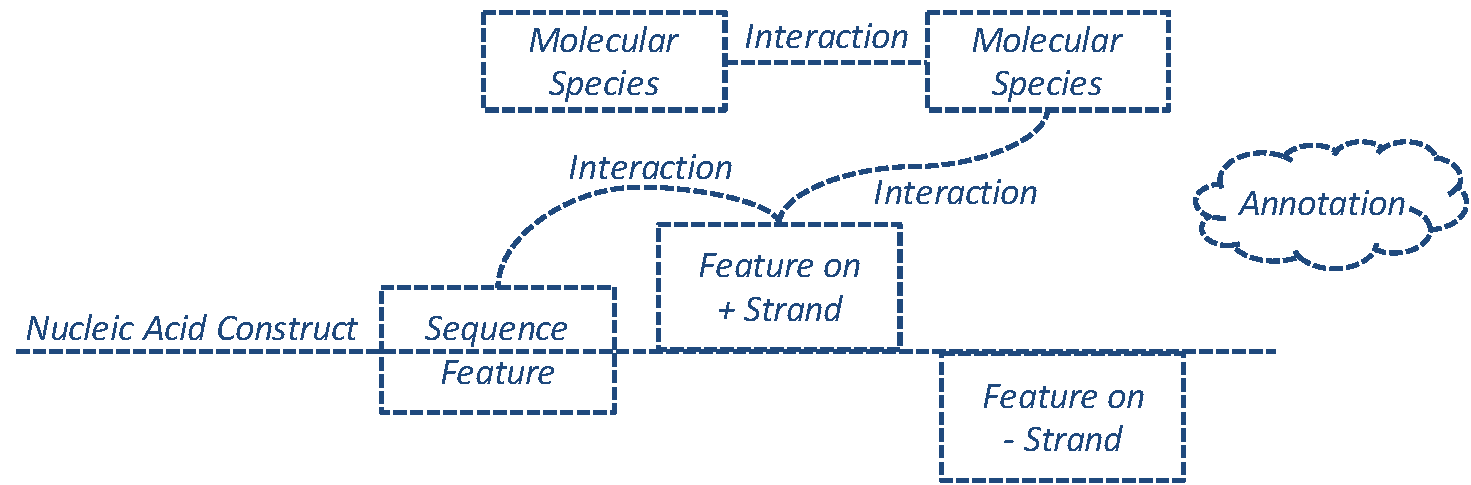
\includegraphics[width=6in]{figures/SBOLsyntax.pdf}
\caption{Generic syntax of SBOL Visual 2:  
a diagram for a nucleic acid construct is based around a backbone line, its structure specified by the sequence of attached sequence feature glyphs.  
Strand can optionally be indicated by placing a glyph above or below the backbone.  
Other molecular species are indicated by glyphs not in contact with any backbone.
Interactions are directed edges connecting sequence feature or molecular species glyphs.
Any of these objects may have an associated label showing its name, and the diagram may further include any form of other annotations, including other types of text.}
\label{f:syntax}
\end{figure}

\begin{figure}[h!]
\centering
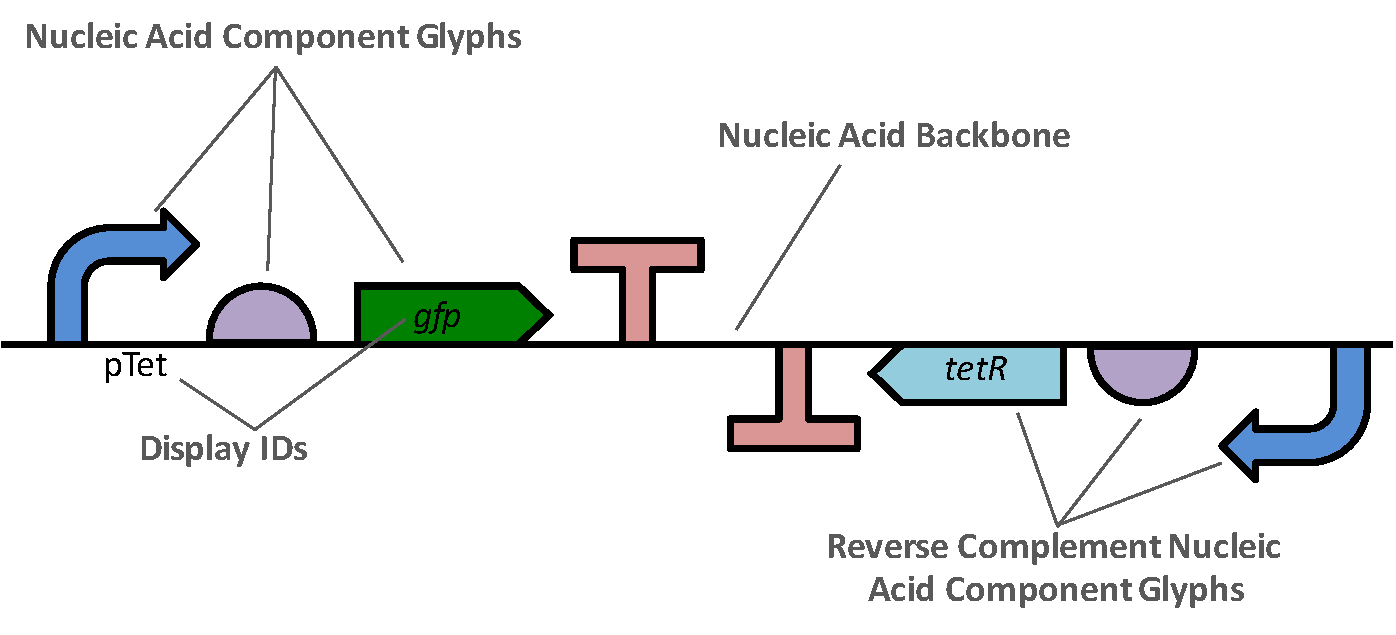
\includegraphics[width=6in]{figures/SBOLgeneral.pdf}
\caption{Example illustrating the elements of an SBOL Visual 2 diagram, with nucleic acid sequence features on the forward and reverse strand of a backbone, other molecular species, and interactions between elements; the grey labels and indicator lines are annotations.}
\label{f:example}
\end{figure}
% inhibition and production relationships

Specifically, an SBOL Visual diagram consists of the classes of objects illustrated in \ref{f:syntax}.
\ref{f:example} shows an example of such a diagram, in a typical usage.
Full details of this specification are provided in the remainder of this section.


\subsection{Nucleic Acid Backbone}
\label{s:lang:backbone}

A diagram for a nucleic acid construct is based around a single or double line, representing the nucleic acid backbone. 
Information about features of the construct can then be represented by attaching nucleic acid glyphs to the backbone, as defined below in \ref{s:lang:nacomponent}
%
In terms of SBOL 2 data models, the backbone represents a \sbol{ComponentDefinition} with a nucleic acid \sbol{type} (e.g., DNA, RNA), and the features represent \sbol{Component} and \sbol{SequenceAnnotation} members of the \sbol{ComponentDefinition}.

\begin{enumerate}
\item Lines in some cases indicate strand count. 
	A double-stranded region of the nucleic acid construct MAY use either a single or double line for the backbone.  
	A single-stranded region of the nucleic acid construct MUST use a single line to indicate the backbone.
	When single and double lines are mixed within a single diagram, the single lines always indicate single-stranded regions.
	Examples are provided in~\ref{exa:1a}.
	
	\begin{figure}[h!]
	\centering
	\subfigure[Single- or double-strand backbone]{
\includegraphics[scale=0.4]{figures/examples/1a-singlestrand.pdf}}
	\subfigure[Double-strand backbone]{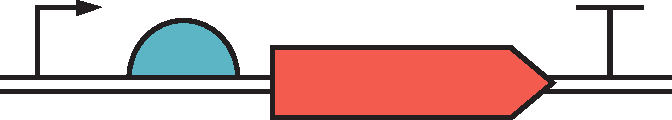
\includegraphics[scale=0.4]{figures/examples/1a-doublestrand.pdf}}
	\subfigure[Double-strand backbone with single-strand overhangs]{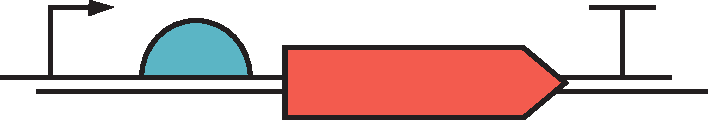
\includegraphics[scale=0.4]{figures/examples/1a-overhangstrand.pdf}}
	\caption{Examples of indicating strand count in nucleic acid backbones.}
	\label{exa:1a}
	\end{figure}
		
\item A nucleic acid backbone SHOULD be horizontal in orientation, 
	but MAY use non-horizontal structure to indicate important physical attributes 
	(e.g., a closed loop to indicate a cyclic plasmid or more complex shapes for DNA nanotech structures).   
	Examples are provided in~\ref{exa:1b}.
	
	\begin{figure}[h!]
	\centering
	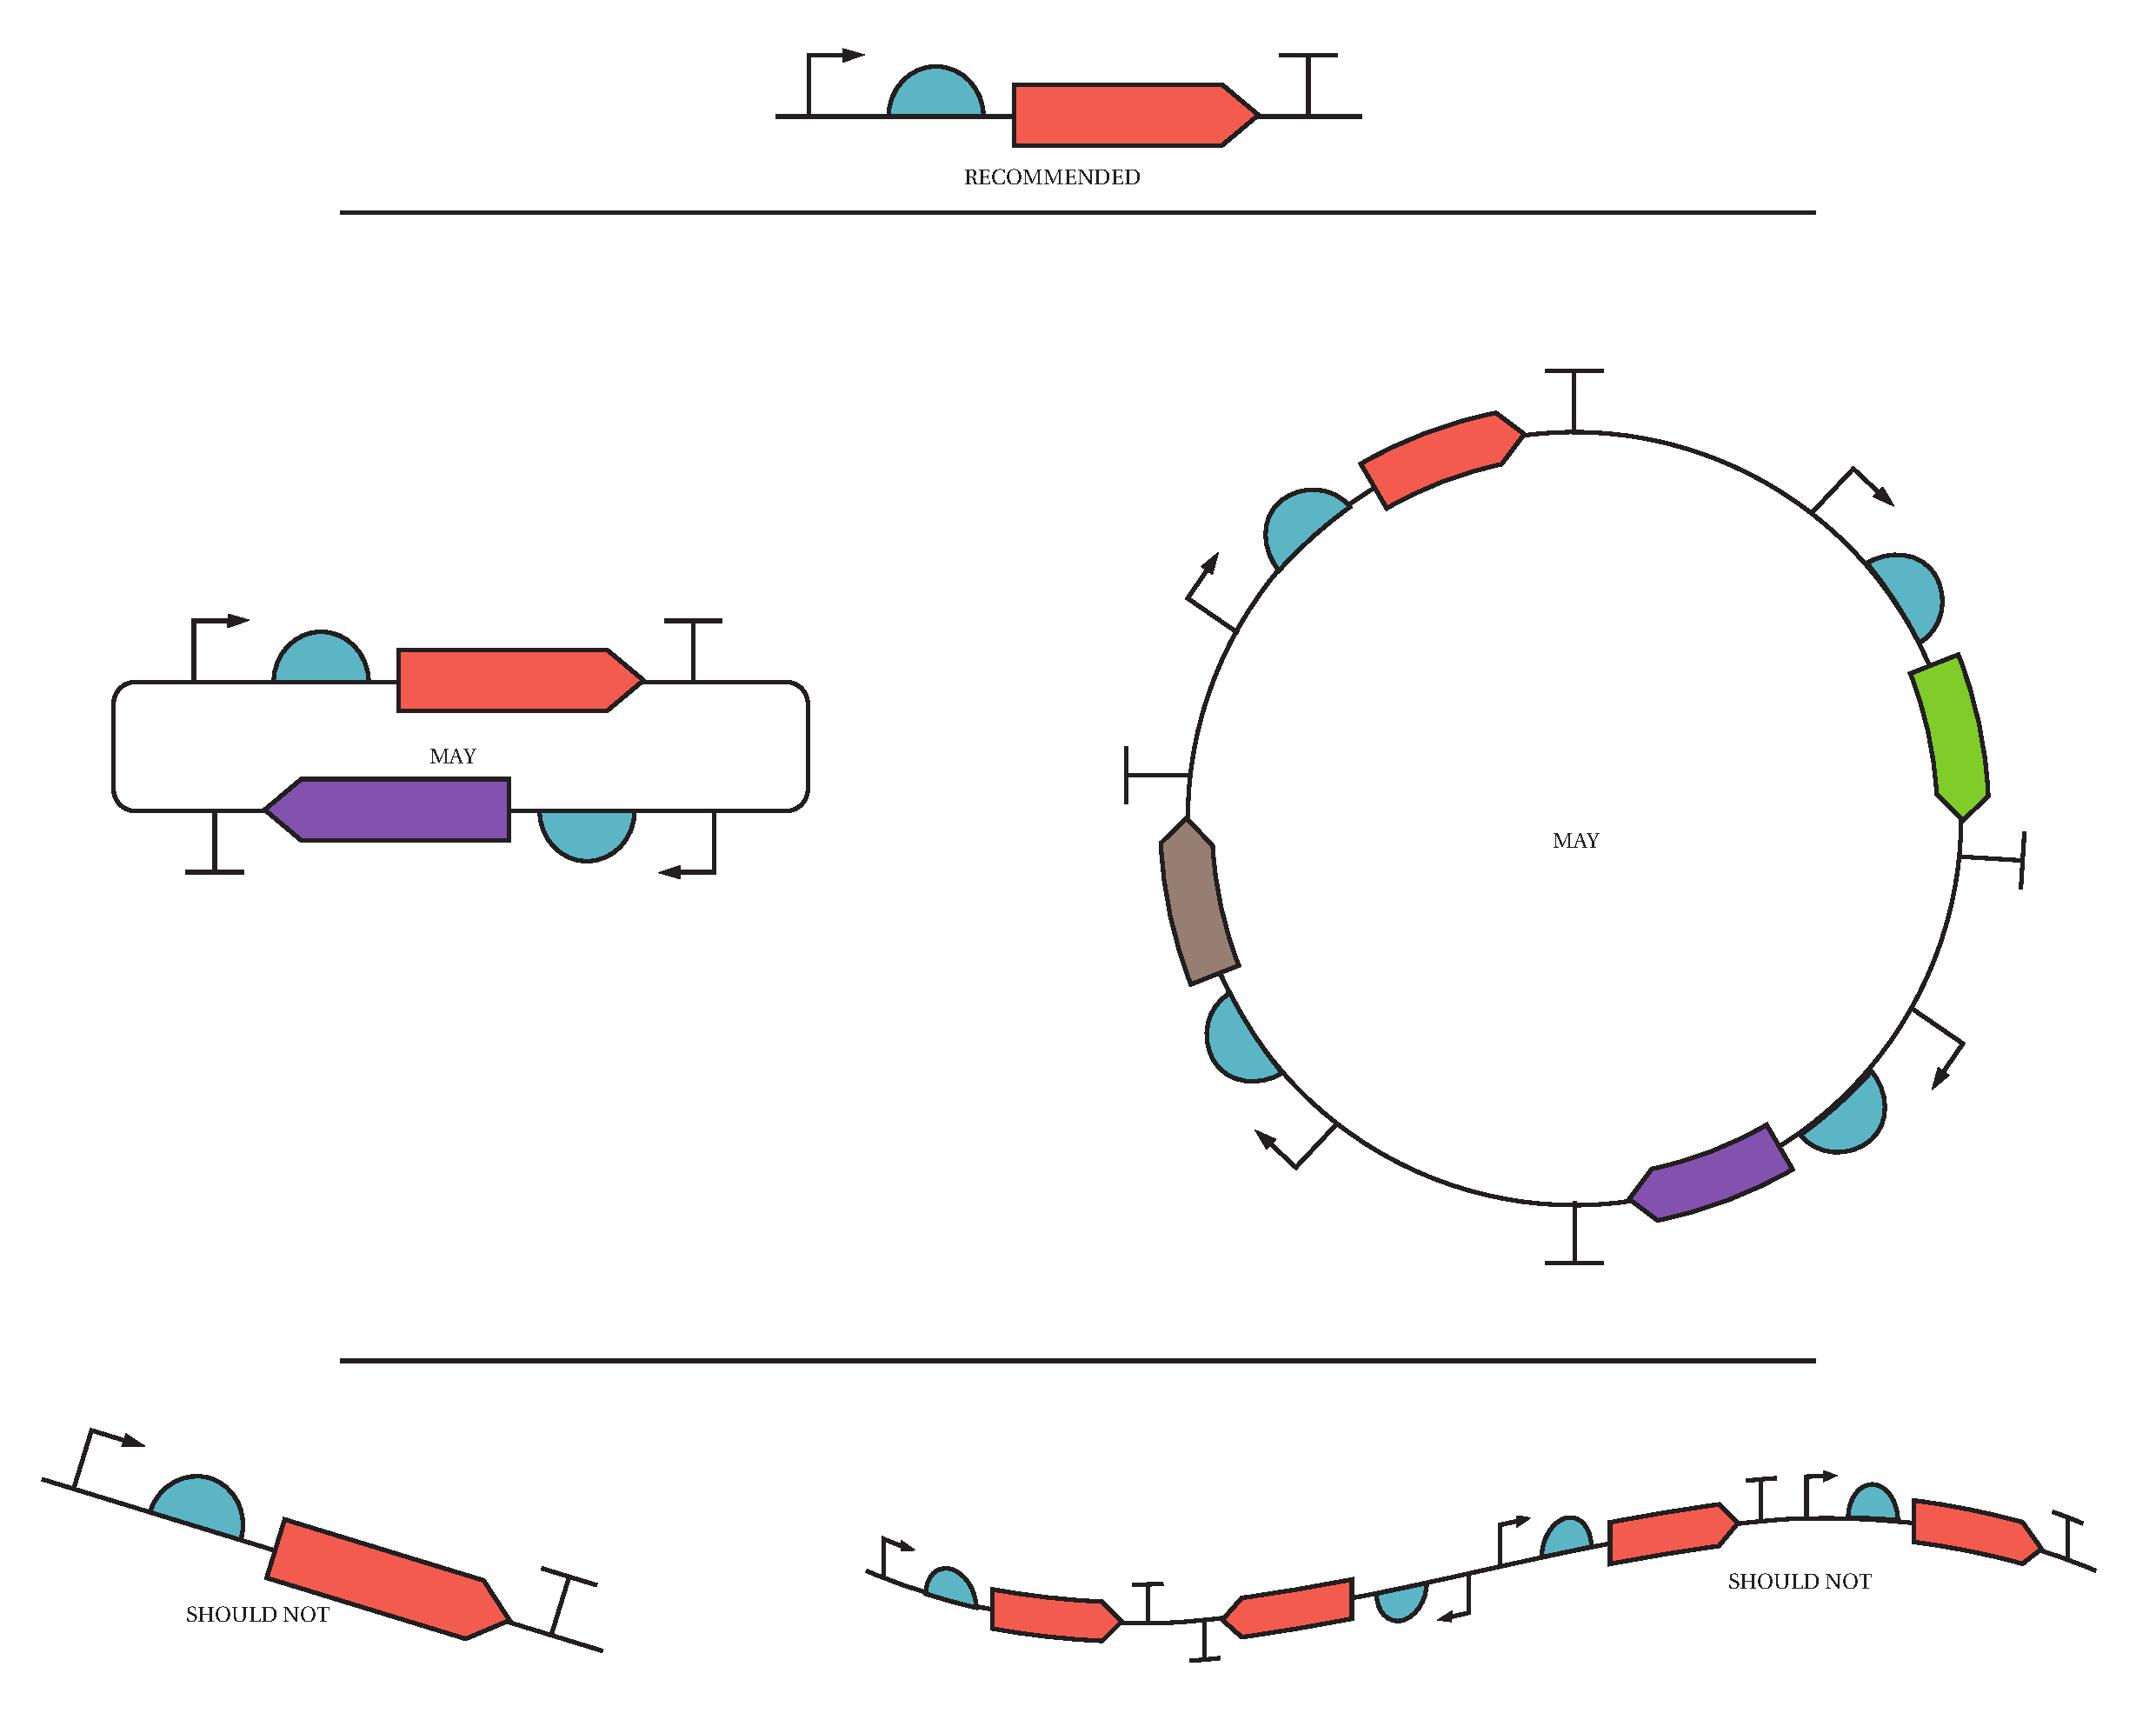
\includegraphics[width=6in]{figures/examples/1b.pdf}
	\caption{Recommended, acceptable, and problematic examples of nucleic backbone orientation.}
	\label{exa:1b}
	\end{figure}
	
\item A nucleic acid backbone SHOULD have at least one associated feature glyph (else no structural information is being provided).
\end{enumerate}


\subsection{Nucleic Acid Sequence Features}
\label{s:lang:nacomponent}

A glyph in contact with a nucleic acid backbone indicates a feature of the nucleic acid sequence.
% 
In terms of SBOL 2 data models, this is either a \sbol{SequenceFeature} or a \sbol{Component} with a nucleic acid \sbol{type} that is contained within the \sbol{ComponentDefinition} associated with that nucleic acid backbone.
The \sbol{Component} may be contained either directly, as one of the \sbol{components} of the \sbol{ComponentDefinition}, or recursively through a sequence of such containments.

\begin{enumerate}
\item Every feature glyph MUST have its bounding box in contact with the backbone for the nucleic acid construct it describes. 
The placement of the glyph SHOULD follow the recommendation for backbone alignment in the glyph specification.
	Examples are provided in~\ref{exa:2a}.
   	\begin{figure}[h!]
	\centering
	\subfigure[MUST]{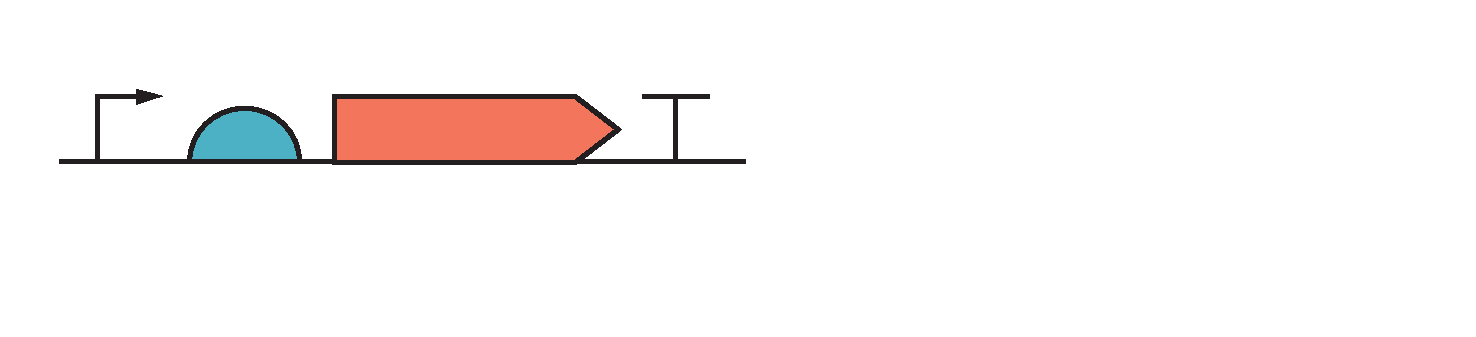
\includegraphics[width=3in]{figures/examples/2a-contact.pdf}}
	\subfigure[MUST NOT]{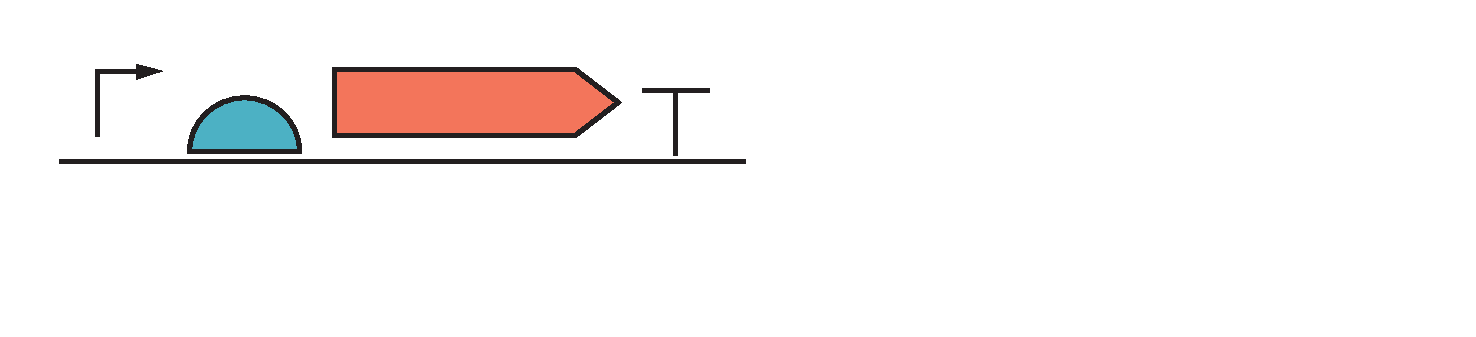
\includegraphics[width=3in]{figures/examples/2a-noncontact.pdf}}
	\caption{Examples of correct and incorrect association of glyphs with a nucleic acid backbone.}
	\label{exa:2a}
	\end{figure}

\item The horizontal orientation of a glyph can be used to indicate the strand alignment of a feature, as shown in \ref{f:orientation}. 
	Any glyphs for a feature associated with the inline strand SHOULD be placed in the prototypical orientation given by the specification,
	while any glyph that is associated with the reverse complement strand SHOULD be inverted vertically and horizontally (i.e., rotated 180 degrees). 
	Reverse complement MAY also be indicated by horizontal-only inversion.
	Finally, a glyph inverted only vertically still indicates inline strand, but it is RECOMMENDED NOT to use this orientation.
	Orientation SHOULD be used consistently throughout a diagram, rather than mixing conventions.
	Examples are provided in \ref{exa:2b}.
	
	\begin{figure}[h!]
	\centering
	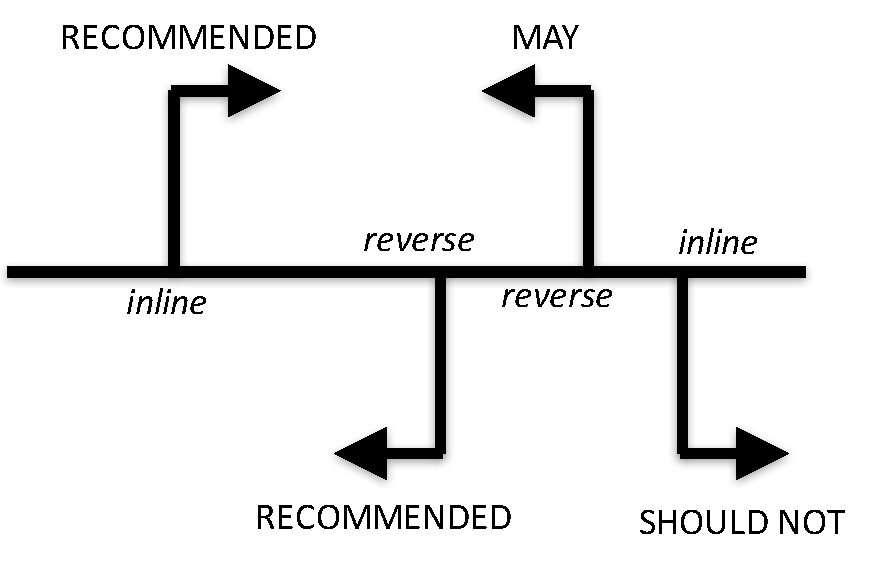
\includegraphics[width=2.5in]{figures/orientation.pdf}
	\caption{Use of glyph orientation to indicate inline vs. reverse complement direction.}
	\label{f:orientation}
	\end{figure} 
	
	\begin{figure}[h!]
	\centering
	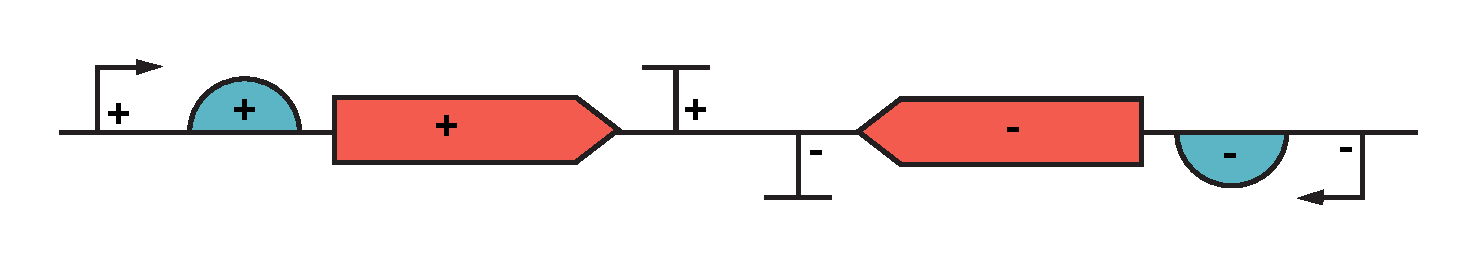
\includegraphics[width=5in]{figures/examples/2b.pdf}
	\caption{Example construct incorporating both inline (+) and reverse complement (-) features.}
	\label{exa:2b}
	\end{figure} 

\item Nucleic acid features in a sequential relationship SHOULD be drawn from 5' left to 3' right on the inline strand and from 5' right to 3' left on the reverse complement strand.
	In terms of SBOL 2 data models, this indicates a \sbol{SequenceConstraint} on the relative ordering of two features.

\item Nucleic acid features that do not overlap in their locations SHOULD NOT have glyphs whose bounding boxes overlap.
	An example is provided in~\ref{exa:2d}.
	\begin{figure}[h!]
	\centering
	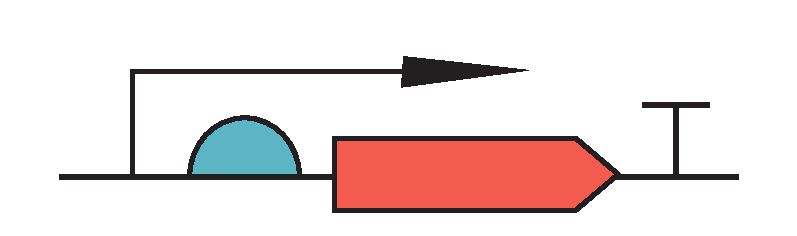
\includegraphics[width=3in]{figures/examples/2d.pdf}
	\caption{Example of incorrect glyph overlap: promoter (arrow) does not overlap in sequence with the ribosome entry site and CDS, so SHOULD NOT overlap visually with them.}
	\label{exa:2d}
	\end{figure}

\item Nucleic acid features that overlap in their locations SHOULD have glyphs whose bounding boxes overlap.  Overlap size MAY be used to indicate relative position.
	Examples are provided in~\ref{exa:2e}.

	\begin{figure}[h!]
	\centering
	\subfigure[Restriction site in a CDS]{
\includegraphics[scale=0.4]{figures/examples/2e-cutsite.pdf}}
	\subfigure[3'-side operator in a promoter]{
\includegraphics[scale=0.4]{figures/examples/2e-promoter.pdf}}
	\subfigure[5'-side operator in a promoter]{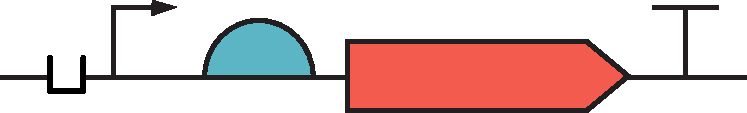
\includegraphics[scale=0.4]{figures/examples/2e-promoter2.pdf}}
	\caption{Examples where glyphs SHOULD overlap, but might not if it is more clear, e.g., with an operator site located within the 5' portion of a promoter.}
	\label{exa:2e}
	\end{figure}

\item A nucleic acid feature SHOULD be represented using a glyph defined in \ref{apdx:sym:feature}.  In this case, the feature MUST be contained within at least one of the glyph's associated terms.
In terms of SBOL 2 data models, this means the glyph is equal to or a parent of at least one of the \sbol{roles} for the \sbol{Component} or its associated \sbol{ComponentDefinition}.
	Moreover, the glyph used SHOULD be the RECOMMENDED variant of the most specific applicable glyph.  Note that novel glyphs not defined in \ref{apdx:sym:feature} MAY be used, but SHOULD be proposed for adoption as described in \ref{sec:extension}.
	Examples are provided in~\ref{exa:2f}.
	\begin{figure}[h!]
	\centering
	\subfigure[SHOULD]{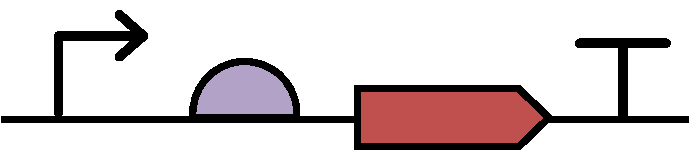
\includegraphics[scale=0.5]{figures/examples/2f-recommended.pdf}}
	\subfigure[MAY]{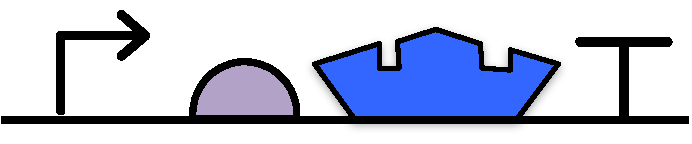
\includegraphics[scale=0.5]{figures/examples/2f-custom.pdf}}
	\subfigure[SHOULD NOT]{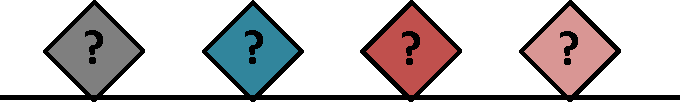
\includegraphics[scale=0.5]{figures/examples/2f-generic.pdf}}
	\subfigure[MUST NOT]{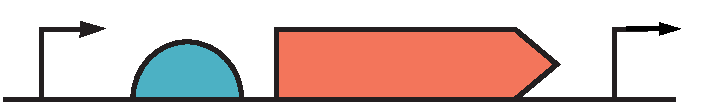
\includegraphics[scale=0.5]{figures/examples/2f-conflict.pdf}}
	\caption{Examples of recommended, allowed, and forbidden representation of a \sbol{ComponentDefinition} comprising a sequence of promoter, ribosome entry site, CDS, and terminator: (a) is RECOMMENDED because it uses the preferred variant of the most specific defined glyphs, (b) is allowed because it uses some novel custom non-conflicting symbol, not matching any glyph defined in this document, to encode more specific information about the particular CDS, (c) is recommended against because it uses less specific glyphs, and (d) is forbidden because it use a promoter symbol to represent the terminator.}
	\label{exa:2f}
	\end{figure}
\end{enumerate}


\subsection{Molecular Species}
A glyph that is not in contact with any backbone represents any class of molecule whose detailed structure is not being shown using sequence feature glyphs.
In other words, either not a nucleic acid (e.g., proteins, small molecules) or else an ``uninteresting'' nucleic acid (e.g., showing a transcribed mRNA, but not the features of its sequence).
In terms of SBOL 2 data models, this is a \sbol{FunctionalComponent} that is contained within a \sbol{ModuleDefinition} implicit in the diagram.

\begin{enumerate}
\item A molecular species glyph MUST NOT contact any nucleic acid backbone with any part of its bounding box.
\item A molecular species SHOULD be represented using a glyph defined in \ref{apdx:sym:species}.  In this case, the species MUST be contained within at least one of the glyph's associated terms.
In terms of SBOL 2 data models, this means the glyph is equal to or a parent of at least one of the \sbol{types} for the associated \sbol{ComponentDefinition}.
	Moreover, the glyph used SHOULD be the RECOMMENDED variant of the most specific applicable glyph.  Note that novel glyphs not defined in \ref{apdx:sym:species} MAY be used, but SHOULD be proposed for adoption as described in \ref{sec:extension}.
\end{enumerate}


\subsection{Interaction}

A directed edge ``arrow'' attached to one or more glyphs indicates a functional interaction involving those elements.
The roles of the elements is indicated by their position at the head or tail of the edge.
In terms of SBOL 2 data models, this is an \sbol{Interaction}, with either one or two \sbol{Participation} relationships, their \sbol{role} set by position at the head or tail of the edge.
	An example is provided in~\ref{exa:4}.

	\begin{figure}[h!]
	\centering
	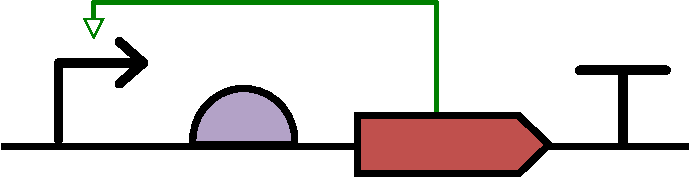
\includegraphics[width=3in]{figures/examples/4-regulation.pdf}
	\caption{Example of an interaction indicating a promoter stimulated by the CDS that it regulates.}
	\label{exa:4}
	\end{figure}
		
\begin{enumerate}
\item Two interaction edges SHOULD NOT cross one another.  When edges cross, they MUST indicate the distinction between arrows with a crossover pattern, in which one edge ``diverts'' at the intersection (see \ref{f:crossover}).
Examples are provided in~\ref{exa:4c}.

	\begin{figure}[h!]
	\centering
	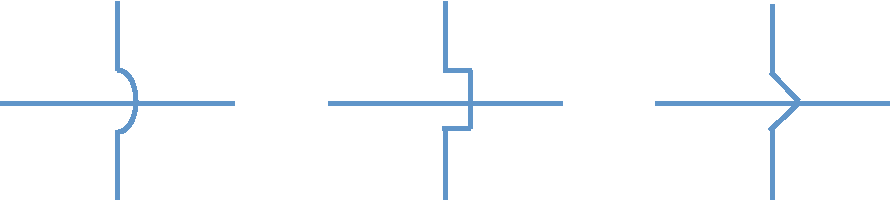
\includegraphics[width=4in]{figures/crossovers.pdf}
	\caption{Examples of \sbol{Interaction} crossover patterns.}
	\label{f:crossover}
	\end{figure}
	
	\begin{figure}[h!]
	\centering
	\subfigure[SHOULD]{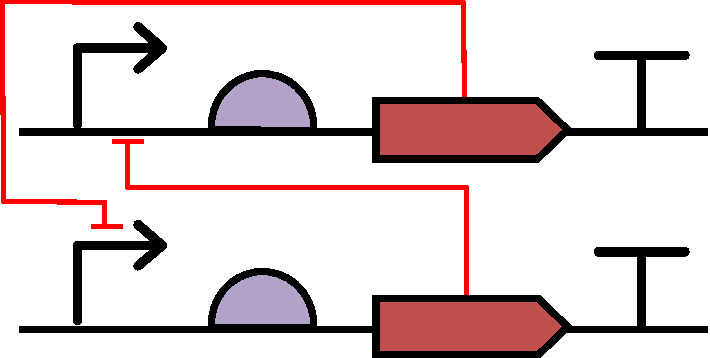
\includegraphics[scale=0.4]{figures/examples/4c-noncrossing.pdf}}
	\subfigure[MAY]{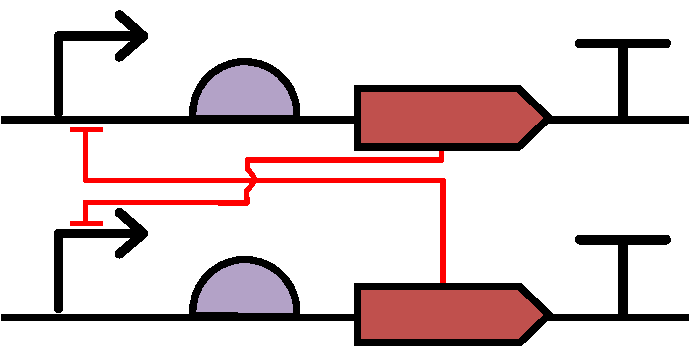
\includegraphics[scale=0.4]{figures/examples/4c-crossover.pdf}}
	\subfigure[MUST NOT]{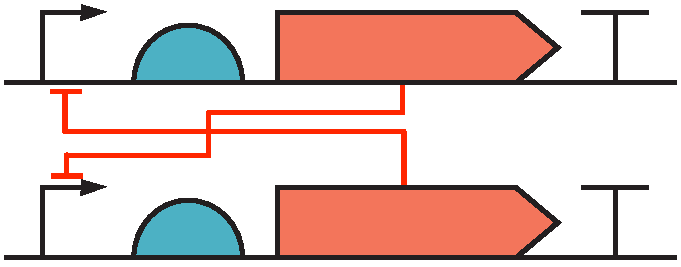
\includegraphics[scale=0.4]{figures/examples/4c-conflict.pdf}}
	\caption{Examples of recommended, allowed, and forbidden relationships between two interactions in a mutual repression system: (a) non-crossing is recommended, (b) using a crossover pattern is allowed, but (c) crossing without a crossover pattern is forbidden, since the relationship between the two edges is ambiguous.}
	\label{exa:4c}
	\end{figure}

\item An interaction SHOULD be represented using a glyph defined in \ref{apdx:sym:interaction}.  In this case, the interaction type MUST be contained within at least one of the glyph's associated terms.
In terms of SBOL 2 data models, this means the glyph is equal to or a parent of at least one of the \sbol{types} for the \sbol{Interaction}, and that each associated \sbol{Participation} object has a \sbol{role} compatible with its position on the head or tail of the edge.
	Moreover, the glyph used SHOULD be the RECOMMENDED variant of the most specific applicable glyph.  Note that novel glyphs not defined in \ref{apdx:sym:interaction} MAY be used, but SHOULD be proposed for adoption as described in \ref{sec:extension}.
\end{enumerate}


\subsection{Labels}
The name of any object in a diagram is RECOMMENDED to be displayed as text within, adjacent to, or otherwise clearly visually connected to the object's associated glyph.  In terms of SBOL 2 data models, this is the \sbol{name} property, and if no \sbol{name} is supplied then the \sbol{displayId} MAY be used instead.
Examples are provided in~\ref{exa:5}.

	\begin{figure}[h!]
	\centering
	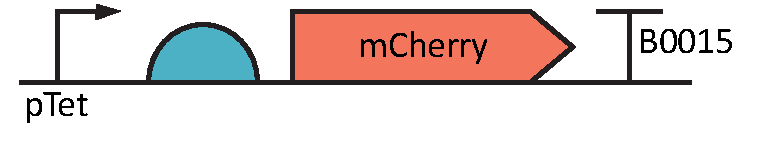
\includegraphics[width=3in]{figures/examples/5-labels.pdf}
	\caption{Examples of labels on glyphs.}
	\label{exa:5}
	\end{figure}


\subsection{Annotations}
Other text or graphics may be included as annotations with no constraint on their syntax or semantics.

\begin{enumerate}
\item Annotations SHOULD NOT be displayed in a way that allows them to be confused with other SBOL Visual elements.
\item Annotations SHOULD NOT be used to display information that can be displayed using other SBOL Visual elements.
\end{enumerate}

\subsection{Criteria for Compliance with SBOL Visual}

A diagram of a biological system is compliant with SBOL Visual if it complies with all MUST and MUST NOT requirements as specified above.
A diagram is compliant with SBOL Visual best practices if it also complies with all RECOMMENDED, SHOULD, and SHOULD NOT statements as specified above.

Importantly, note that a non-SBOL glyph can be used in a compliant
diagram when its definition is a subset or superset of a definition that
does have an SBOL Visual glyph.  For example, a diagram that creates a
new glyph for a special type of promoter can be SBOL Visual compliant
even though there is an SBOL Visual glyph for a general promoter.

A piece of software or other system for producing diagrams is
compliant with SBOL Visual under the following conditions:
\begin{enumerate}
\item The system MUST be capable of producing diagrams that are
  compliant with SBOL Visual.
\item If the system can also produce diagrams that are {\em not}
  compliant with SBOL Visual, it MUST clearly distinguish to the user
  between compliant and non-compliant usage and diagrams.
\end{enumerate}

